\documentclass[tikz]{standalone}

\usepackage{amsmath}
\usepackage{unicode-math}
\usepackage{mathtools}
\usepackage{derivative}

\setmainfont{Stix Two Text}
\setmathfont{Stix Two Math}

\usetikzlibrary{arrows.meta,fit,positioning}

\renewcommand{\familydefault}{\sfdefault}

% prefix equation numbers with section number
\numberwithin{equation}{section}

\DeclarePairedDelimiter{\ceil}{\lceil}{\rceil}
\DeclarePairedDelimiter{\floor}{\lfloor}{\rfloor}
\DeclarePairedDelimiter{\abs}{\lvert}{\rvert}
\DeclarePairedDelimiter{\norm}{\lVert}{\rVert}
\DeclarePairedDelimiter{\bra}{\langle}{\rvert}
\DeclarePairedDelimiter{\ket}{\lvert}{\rangle}
\DeclarePairedDelimiter{\expval}{\langle}{\rangle}
\DeclarePairedDelimiter{\norder}{\mathcolon}{\mathcolon}
\DeclarePairedDelimiter{\anorder}{\typecolon}{\typecolon}
	
\newcommand{\laplace}{\mbfnabla^2}
\newcommand{\trans}{{\scriptscriptstyle\mathsf{T}}}

\newcommand{\vdot}{\cdot}
\newcommand{\vcross}{\vectimes}
\newcommand{\vb}[1]{\symbfup{#1}}
\newcommand{\vu}[1]{\hat{\vb{#1}}}
\newcommand*\dd[2][\relax]{\mathop{\ifx\relax#1\odif{#2}\else \odif[order={#1}]{#2}\fi\,}}

\newcommand{\vacuum}{\ket*{\vb{0}}}

\DeclareMathOperator{\trace}{Tr}
\DeclareMathOperator{\sinc}{sinc}

\AtBeginDocument{
	\let\Re\relax
	\let\Im\relax
	\DeclareMathOperator{\Re}{Re}
	\DeclareMathOperator{\Im}{Im}

	\renewcommand{\div}{\mathop{\mbfnabla\vdot}}
	\newcommand{\curl}{\mathop{\mbfnabla\vectimes}}
}

\DeclarePairedDelimiterX{\comm}[2]{[}{]}{#1,#2}

\DeclarePairedDelimiterX{\braket}[2]{\langle}{\rangle}{#1\delimsize\vert#2}
\DeclarePairedDelimiterX{\ketbra}[1]{\lvert}{\rvert}{#1\rangle\delimsize\langle#1}



\begin{document}
	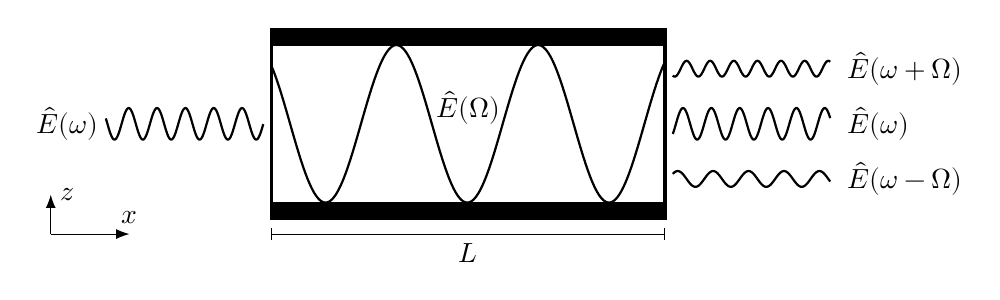
\begin{tikzpicture}[
		electrode/.style={fill=black},
		waveform/.style={thick},
		label/.style={anchor=west},
	]
		\draw[very thick] (0,-0.2) rectangle ++(5,2.4);
		\draw[electrode] (0,-0.2) rectangle ++(5,0.2);
		\draw[electrode] (0,2) rectangle ++(5,0.2);
		
		\draw[waveform, domain=0:5, samples=500] plot (\x,{1+cos(200*\x+42)});
		\draw[waveform, domain=-2:0, samples=500] plot (\x-0.1,{1+0.2*sin(1000*\x)});
		\draw[waveform, domain=5:7, samples=500] plot (\x+0.1,{1+0.2*sin(1000*\x)});
		\draw[waveform, domain=5:7, samples=500] plot (\x+0.1,{1.7+0.1*sin(1200*\x)});
		\draw[waveform, domain=5:7, samples=500] plot (\x+0.1,{0.3+0.1*sin(800*\x)});
		
		\draw[Bar-Bar] (0,-0.4) -- ++(5,0) node[midway, below] {$L$};
		
		\coordinate (origin) at (-2.8,-0.4);
		\draw[-Latex] (origin) -- ++(1,0) node[above] {$x$};
		\draw[-Latex] (origin) -- ++(0,0.5) node[right] {$z$};
		
		\node[label] at (-3.1,1) {$\hat{E}(\omega)$};
		\node[label] at (7.2,1) {$\hat{E}(\omega)$};
		\node[label] at (7.2,1.7) {$\hat{E}(\omega+\Omega)$};
		\node[label] at (7.2,0.3) {$\hat{E}(\omega-\Omega)$};
		
		\node at (2.5,1.2) {$\hat{E}(\Omega)$};
	\end{tikzpicture}
\end{document}
